\section{Life course of intimate relationships}
\label{sec:life_course}
Levy \cite{levy2014intimate} defined a so called \textit{life course of intimate relationships}. This course includes four conditions of romantic relationships as can be seen in figure \ref{fig:live_course}. The colors from the figure \ref{fig:cluster} are taken up here and reproduced in the individual conditions. The connection to the individual topics should be roughly indicated. The transitions in the content can be fluid.
\begin{figure}[htb]
    \centering
	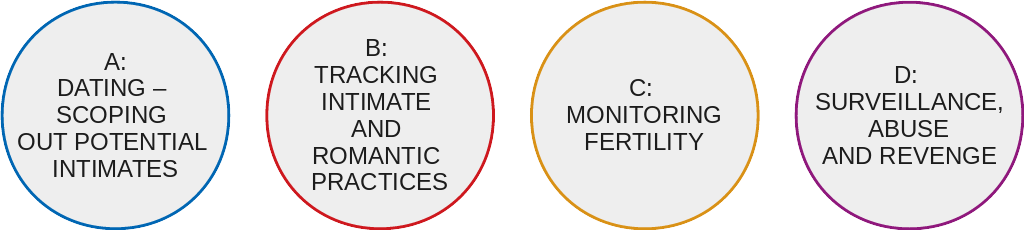
\includegraphics[width=\linewidth]{img/life_course.png}
	\caption{The life course of intimate surveillance (based on the work by Levy \cite{levy2014intimate}).}
	\label{fig:live_course}
\end{figure}

In each of these conditions technologies can be used for different purposes.

Condition \textbf{A} stands for the beginning of a potential relationship. The partners know each other or would like to know each other. At this point, there is an interest from one or both sides. The aim is to learn more about the other person, to check their identity and social life.

In condition \textbf{B} the partners are already in a relationship or something appropriate. At this point, it should be emphasized that this condition includes all sorts of relationships that are understood as such. For a concrete definition what a romantic relationship means see Danaher et al. \cite{doi:10.1080/15265161.2017.1409823}. In this condition the partners know each other better and have an increased (mutual) interest. There are other forms of interests against the other, possibly sexual ones.

In condition \textbf{C} there is usually an established relationship (but that does not have to be the case). The couple exercises sexual activities, deals with contraceptive measures (together) or plans to start a family.

Condition \textbf{D} stands for the surveillance in a relationship, also abuse and revenge. This condition is sort of difficult to explain. 
The relationship may already be over. Then the partners have a relationship to each other based on their previous history. The condition D is about surveillance, abuse and revenge. Surveillance in a relationship may be voluntary and knowingly, accepted by the partners, or unknowingly, in unawareness of the monitored partner.
This condition maybe arise from problems in the relationship, due to interpersonal conflicts oder something else.

Since relationships are complex and individual \cite{sassler2010partnering}, the single conditions are not interconnected . Also this is not the focus of this work. The descriptions above only should give an idea of what the conditions mean for the following section \ref{sec:consideration_life_course_conditions}.
